\documentclass[10pt,a4paper]{article}
\usepackage[margin=2.2cm]{geometry}
\usepackage{amsmath,amssymb,graphicx,booktabs,siunitx}
\usepackage[hidelinks]{hyperref}
\usepackage[font=small,labelfont=bf]{caption}
\usepackage{microtype}
\graphicspath{{../figures/}}
\newcommand{\ee}{\mathrm{e}}
\newcommand{\ii}{\mathrm{i}}

\title{\textbf{Equivalent Robin coefficients for porous acoustic absorbers:\\closed form, frequency regimes and nonlocal error}}
\author{Minka Dubourg}
\date{October 2024}

\begin{document}
\maketitle

\begin{abstract}
\noindent
Replacing a porous absorbing wall by a Robin boundary condition $\eta_0\partial_\nu u+\alpha(\omega)u=0$ removes the need to mesh the wall. We compute the coefficient $\alpha^*(\omega)$ that best reproduces the full air--wall transmission problem, using the modal error functional of Magoulès \textit{et al.}~\cite{magoules2021}, for three materials (melamine foam, ISOREL, Birch LT) and two source geometries. Four findings emerge.
(i)~For a plane wave, the optimum is exactly $\alpha^*=\eta_1\lambda_1(0,\omega)$, the wall's Dirichlet-to-Neumann symbol at normal incidence. The numerical optimum matches it to $10^{-7}$, and the residual vanishes to round-off.
(ii)~$\alpha^*$ crosses over from a viscous regime, $\alpha^*\propto(1-\ii)\sqrt{\omega}$, to an inertial regime with saturating real part, at $\omega_c=\sigma\phi/(\rho_0\alpha_h)$.
(iii)~For spatially structured sources, the wall's response is nonlocal in $y$, so no constant $\alpha$ is exact. The residual error ranges from $10^{-6}$ to $10^{-3}$ and is ordered by the nonlocality parameter $k_\mathrm{eff}^2/|\kappa_1^2|$.
(iv)~The optimal coefficient is independent of the source's frequency envelope. Minimising the raw functional without normalising by the source energy breaks this invariance and yields spurious, non-physical coefficients.
\end{abstract}

\section{Introduction}
Predicting sound levels in rooms, ducts or engine nacelles lined with porous material requires coupling the Helmholtz equation in air with a dissipative model inside the liner. Meshing the liner is costly, especially when its placement is itself being optimised~\cite{magoules2024}. A standard reduction keeps only the air domain and represents the liner by an impedance-type boundary condition, $\eta_0\partial_\nu u+\alpha u=0$ on the wall~\cite{allard2009}.

Two questions then arise: which $\alpha$ to use, and how much accuracy the reduction loses. Magoulès \textit{et al.}~\cite{magoules2021} define $\alpha(\omega)$ as the minimiser of the $H^1$-type distance between the solutions of the full and reduced problems, and give a closed-form modal expression for that distance. This note uses that formulation and makes three contributions. First, it identifies the optimum analytically in the plane-wave case and characterises its frequency regimes. Second, it quantifies the irreducible error when the source has spatial structure, and links it to the nonlocality of the wall's response. Third, it documents a normalisation issue that otherwise corrupts the numerical optimum. All results are reproducible from the accompanying code.

\section{Model}
\paragraph{Geometry and equations.}
Let $\Omega=(-L,L)\times(-\ell,\ell)$, with air in $\Omega_\mathrm{air}=\{x<0\}$, the porous wall in $\Omega_\mathrm{wall}=\{x>0\}$, and interface $\Gamma=\{x=0\}$. The source $g(y)$ is imposed at $x=-L$, and the problem is periodic in $y$. In the frequency domain, the full problem reads
\begin{align}
-\nabla\!\cdot(\eta_0\nabla u_0)-\omega^2\xi_0u_0&=0 &&\text{in }\Omega_\mathrm{air},\\
-\nabla\!\cdot(\eta_1\nabla u_1)-\omega^2\xi_1\Big(1+\frac{\ii a}{\xi_1\omega}\Big)u_1&=0 &&\text{in }\Omega_\mathrm{wall},\label{eq:wall}
\end{align}
with continuity of $u$ and of $\eta\,\partial_\nu u$ across $\Gamma$, and $u_0(-L,y)=g(y)$. The reduced problem keeps only the air equation, for $u_2$, with the Robin condition $\eta_0\partial_\nu u_2+\alpha u_2=0$ on $\Gamma$. Here $\eta_0=1$ and $\xi_0=1/c_0^2$. The wall coefficients come from a rigid-frame model~\cite{allard2009} with porosity $\phi$, flow resistivity $\sigma$ and tortuosity $\alpha_h$:
\[
\eta_1=\frac{\phi}{\alpha_h},\qquad \xi_1=\frac{\phi\gamma_p}{c_0^2},\qquad a=\frac{\sigma\phi^2\gamma_p}{c_0^2\rho_0\alpha_h}.
\]

\paragraph{Modal error functional.}
Expanding in Fourier modes $k=n\pi/\ell$ with coefficients $g_k$, the distance $A\|u_0-u_2\|^2_{L^2}+B\|\nabla(u_0-u_2)\|^2_{L^2}$ over $\Omega_\mathrm{air}$ becomes $e(\alpha,\omega)=\sum_k e_k(\alpha,\omega)$~\cite{magoules2021}. Each $e_k$ is a closed-form function of the decay rates
\[
\lambda_0=\sqrt{k^2-\xi_0\omega^2/\eta_0}\ \ (\text{or } \ii\sqrt{\xi_0\omega^2/\eta_0-k^2}),\qquad
\lambda_1=\sqrt{k^2+\kappa_1^2},\quad \kappa_1^2=-\frac{\omega^2\xi_1}{\eta_1}\Big(1+\frac{\ii a}{\xi_1\omega}\Big),
\]
where $\lambda_1$ is taken on the branch with $\operatorname{Re}\lambda_1>0$ and $\operatorname{Im}\lambda_1<0$. It also depends on the two amplitudes
\[
\chi_k=g_k\Big[\frac{\lambda_0\eta_0-\lambda_1\eta_1}{f(\lambda_1\eta_1)}-\frac{\lambda_0\eta_0-\alpha}{f(\alpha)}\Big],\qquad
\gamma_k=g_k\Big[\frac{\lambda_0\eta_0+\lambda_1\eta_1}{f(\lambda_1\eta_1)}-\frac{\lambda_0\eta_0+\alpha}{f(\alpha)}\Big],
\]
with $f(x)=(\lambda_0\eta_0-x)\ee^{-\lambda_0L}+(\lambda_0\eta_0+x)\ee^{\lambda_0L}$. We use $A=B=1$, $L=\ell=2$~m, and $|n|\le20$. Table~\ref{tab:mat} lists the materials.

\begin{table}[h]\centering\small
\begin{tabular}{lrrrr}\toprule
Material & $\phi$ & $\sigma$ (N\,s\,m$^{-4}$) & $\alpha_h$ & $\omega_c$ (rad/s)\\\midrule
Melamine foam & 0.99 & \num{14000} & 1.02 & \num{1.1e4}\\
Birch LT & 0.529 & \num{151429} & 1.37 & \num{4.9e4}\\
ISOREL & 0.70 & \num{142300} & 1.15 & \num{7.2e4}\\\bottomrule
\end{tabular}
\caption{Material parameters and viscous--inertial crossover frequency $\omega_c=\sigma\phi/(\rho_0\alpha_h)$. Air: $\rho_0=1.2$~kg/m$^3$, $c_0=340$~m/s, $\gamma_p=7/5$.}\label{tab:mat}
\end{table}

\section{Method}
\paragraph{Normalised objective.} Since $\chi_k$ and $\gamma_k$ are linear in $g_k$, $e$ is quadratic in the source. We therefore minimise
\[
\alpha^*(\omega)=\arg\min_{\alpha\in\mathbb C}\ \frac{e(\alpha,\omega)}{\sum_k|g_k|^2},
\]
which is invariant under any rescaling $g\mapsto s(\omega)g$. Section~\ref{sec:norm} shows why this matters numerically.

\paragraph{Optimisation.} The objective is minimised over $(\operatorname{Re}\alpha,\operatorname{Im}\alpha)$ by Nelder--Mead from several starting points. Along a frequency sweep, the start set also includes the previous frequency's optimum (warm start). The $e_k$ are evaluated in vectorised form over $k$. The coefficients $g_k$ are computed once by quadrature, since they do not depend on $\alpha$.

\paragraph{Sources.} We use a uniform source $g\equiv1$, which is a plane wave exciting only $k=0$, and a Gaussian beam $g(y)=\ee^{-y^2}$, whose spectral weight is spread over $k$ with $k_\mathrm{eff}^2=\sum_k k^2|g_k|^2/\sum_k|g_k|^2\approx1.0$~m$^{-2}$. We sweep 400 frequencies with $\omega\in[10^2,3\times10^4]$~rad/s.

\section{Results}
\subsection{Plane wave: an exact closed form}
Setting $\alpha=\lambda_1\eta_1$ makes the two terms in $\chi_k$ and in $\gamma_k$ identical, so $\chi_k=\gamma_k=0$ and $e_k=0$. This has a direct interpretation. For a single mode, the wall solution decays as $\ee^{-\lambda_1x}$, so $\eta_1\partial_xu_1=-\eta_1\lambda_1u_1$ on $\Gamma$, and $\eta_1\lambda_1(k,\omega)$ is the exact Dirichlet-to-Neumann symbol of the wall. A plane wave contains only $k=0$, so
\[
\alpha^*(\omega)=\eta_1\lambda_1(0,\omega).
\]
The numerical optimum reproduces this to a relative $10^{-7}$ for all materials and frequencies, with a residual below $5\times10^{-13}$ (Fig.~\ref{fig:alpha}). This also validates the implementation of $e_k$ independently.

\begin{figure}[t]\centering
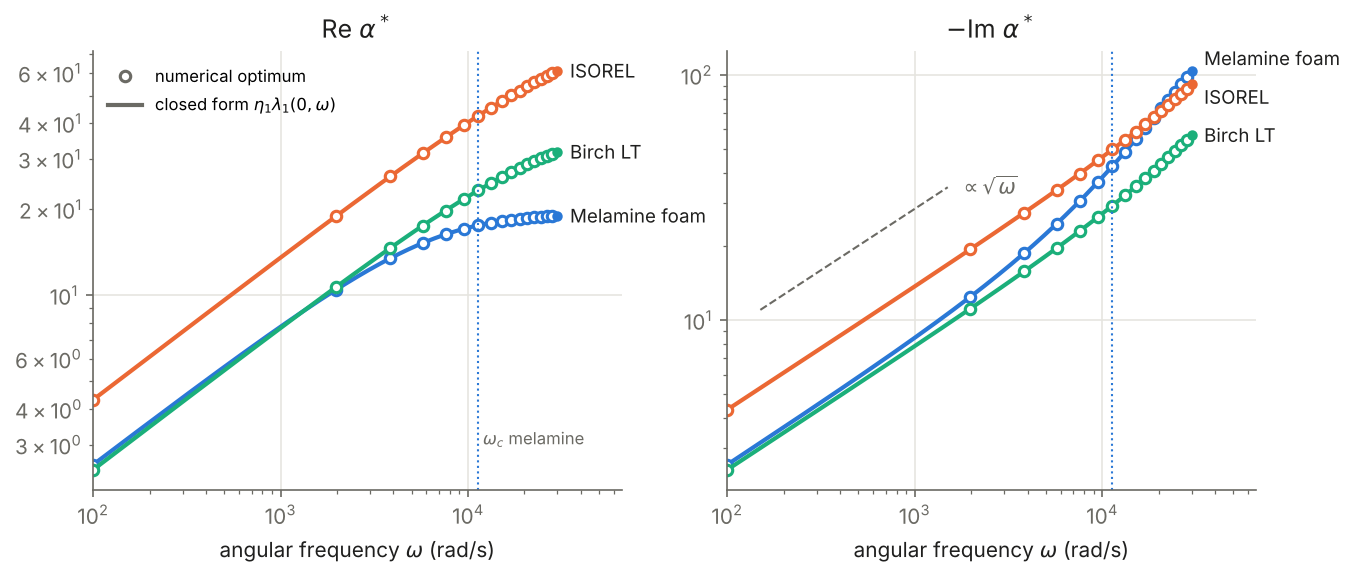
\includegraphics[width=\textwidth]{alpha_vs_omega.png}
\caption{Optimal coefficient for a plane-wave source. Circles: numerical optimum. Lines: closed form $\eta_1\lambda_1(0,\omega)$. The dotted line marks $\omega_c$ for melamine.}\label{fig:alpha}
\end{figure}

\subsection{Two frequency regimes}
Writing $\eta_1\lambda_1(0,\omega)=\eta_1\sqrt{-\omega^2\xi_1/\eta_1-\ii a\omega/\eta_1}$ separates two limits, at $\omega_c=a/\xi_1=\sigma\phi/(\rho_0\alpha_h)$:
\[
\omega\ll\omega_c:\ \ \alpha^*\simeq(1-\ii)\sqrt{\tfrac{a\eta_1\omega}{2}},\qquad
\omega\gg\omega_c:\ \ \alpha^*\simeq\tfrac a2\sqrt{\tfrac{\eta_1}{\xi_1}}-\ii\,\omega\sqrt{\xi_1\eta_1}.
\]
In the viscous regime, the real and imaginary parts are equal in magnitude and grow as $\sqrt\omega$. In the inertial regime, the dissipative part saturates and the reactive part grows linearly. At $\omega=100$~rad/s, the low-frequency asymptote is accurate to better than $0.5\%$. Melamine crosses over inside the sweep: $\operatorname{Re}\alpha^*$ reaches $19.0$ at $3\times10^4$~rad/s against the limit $19.3$. ISOREL and Birch LT have $\omega_c$ above the sweep and remain mostly viscous.

\subsection{Structured sources: the error of a local condition}
A Gaussian beam excites many modes, each of which would require its own $\alpha_k=\eta_1\lambda_1(k,\omega)$. A constant $\alpha$ is a local approximation of a nonlocal operator, and it cannot be exact. The optimum is a compromise weighted by $|g_k|^2$. It stays within $1.4\%$ (melamine) and $0.25\%$ (ISOREL, Birch LT) of the plane-wave value. The largest deviation occurs near $\omega\approx1.9\times10^3$~rad/s for all three materials, which suggests an air-side rather than material origin.

Because $\lambda_1=\sqrt{k^2+\kappa_1^2}$, the relative variation of the symbol across the source spectrum scales as $k_\mathrm{eff}^2/|\kappa_1^2|$. At $\omega=3\times10^3$~rad/s this is $2.3\times10^{-3}$ for melamine, against $3$--$4\times10^{-4}$ for ISOREL and Birch LT. The ratio decreases with frequency as $|\kappa_1^2|$ grows. This orders the residual error correctly: melamine, the least resistive material, has the most nonlocal response and the largest error (Fig.~\ref{fig:res}).

\begin{figure}[t]\centering
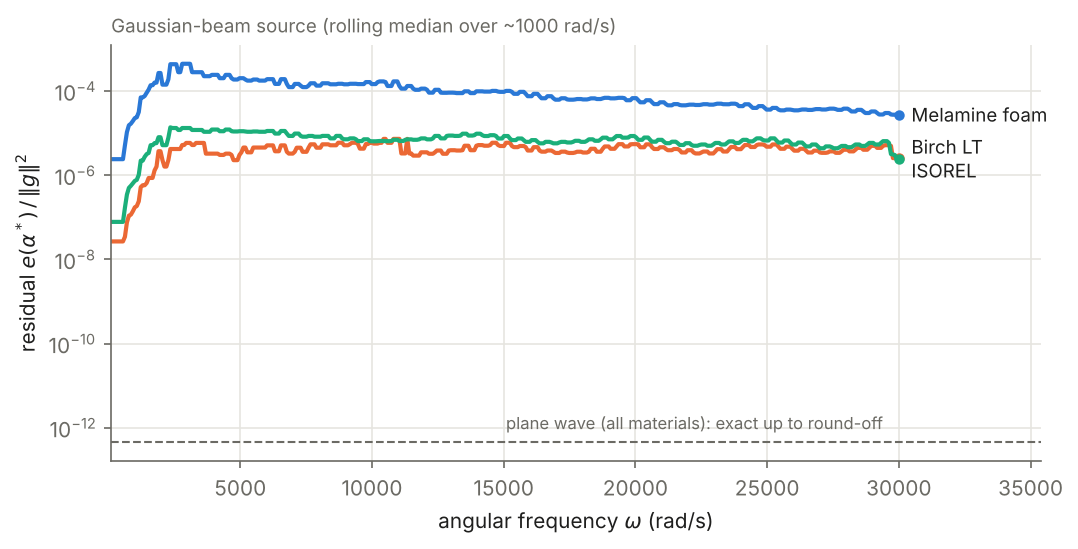
\includegraphics[width=0.78\textwidth]{residual_gaussian_beam.png}
\caption{Normalised residual $e(\alpha^*)/\|g\|^2$ for a Gaussian-beam source (rolling median). Dashed line: the plane-wave residual, which is zero up to round-off.}\label{fig:res}
\end{figure}

\subsection{Why normalisation matters}\label{sec:norm}
The optimal $\alpha$ cannot depend on the amplitude of $g$. A narrow-band source $g(y,\omega)=\ee^{-(\omega-\omega_0)^2/2s^2}$, with $\omega_0=1.5\times10^4$ and $s=10^3$~rad/s, has the same $\alpha^*$ as a plane wave. Minimising the raw $|e|$ instead, here with L-BFGS-B from $\alpha=1+\ii$, fails as soon as the source amplitude, and hence $e$, falls below the optimiser's absolute tolerance. The iteration stops at its starting point, and the returned value has $\operatorname{Im}\alpha>0$, which is non-physical for a passive wall. It also shows spikes at the transition (Fig.~\ref{fig:norm}). In a sweep these artefacts look like physical features, such as absorption concentrated near $\omega_0$ or resonances, but they come only from the optimiser. Normalising by $\sum_k|g_k|^2$ removes them. The test suite checks the amplitude invariance down to scale factors of $10^{-10}$.

\begin{figure}[t]\centering
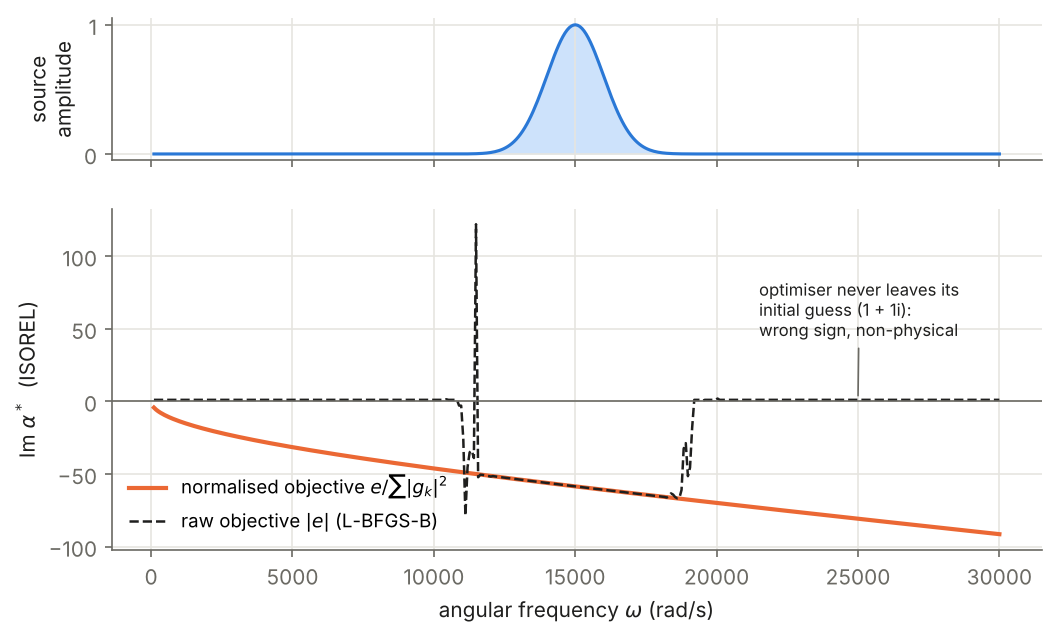
\includegraphics[width=0.72\textwidth]{normalisation_artefact.png}
\caption{Narrow-band source (top) and the resulting $\operatorname{Im}\alpha^*$ for ISOREL (bottom), with and without normalisation.}\label{fig:norm}
\end{figure}

\section{Discussion and limitations}
For plane-wave excitation, the equivalent-condition problem has an exact closed-form answer. Numerical optimisation is only needed for structured sources, and there the error of the local reduction is small and predictable from $k_\mathrm{eff}^2/|\kappa_1^2|$. Practical consequences: resistive liners are well represented by a single $\alpha$, while low-resistivity foams at low frequency are the least suited to a local condition.

Limitations: the wall is modelled as rigid-frame and half-space-like, with a planar interface and $A=B=1$. The residual for structured sources also shows fine structure in $\omega$ that is not resolved here. It is not aligned with the air-side mode cut-offs $\omega_n=n\pi c_0/\ell$, and we have not separated it from optimiser tolerance.

Natural extensions are: a single $\alpha$ optimised over a frequency band, which is the quantity used when optimising liner placement~\cite{magoules2024}; nonlocal (pseudo-differential) boundary conditions built from $\eta_1\lambda_1(k,\omega)$; and comparison with time-domain impedance models.

\paragraph{Code and data.} \url{https://github.com/minkadubourg/porous-wall-impedance}. All figures are produced by \texttt{scripts/compute.py} and \texttt{scripts/make\_figures.py}.

\begin{thebibliography}{9}\small
\bibitem{magoules2021} F.~Magoulès, T.~P.~K.~Nguyen, P.~Omnes, A.~Rozanova-Pierrat. Optimal absorption of acoustic waves by a boundary. \textit{SIAM J. Control Optim.}, 2021. doi:10.1137/20M1327239.
\bibitem{magoules2024} F.~Magoulès, M.~Menoux, A.~Rozanova-Pierrat. Frequency range non-Lipschitz parametric optimization of a noise absorption. arXiv:2409.06292, 2024.
\bibitem{allard2009} J.-F.~Allard, N.~Atalla. \textit{Propagation of Sound in Porous Media}, 2nd ed. Wiley, 2009.
\end{thebibliography}
\end{document}
